\subsubsection*{introduction of the Problem}

\begin{frame}
      \frametitle{Introduction of the Problem}
      
      We use $C_{n}$ to represent a graph look like regular polygons with $n$ vertices.

      \begin{figure}[h!]
            \tikzstyle{vertex}=[circle,fill=black!25,minimum size=20pt,inner sep=0pt]
            \tikzstyle{edge} = [draw,thick,-]
            \tikzstyle{weight} = [font=\small]
            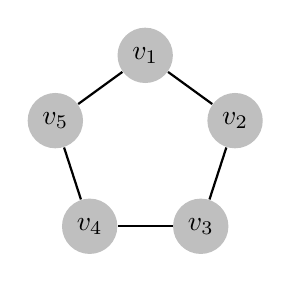
\begin{tikzpicture}[scale=0.6, auto,swap]
                  % Draw a 7,11 network
                  % First we draw the vertices
                  \foreach \pos/\name/\la in {{(0,2)/a/$v_{1}$},
                  {(1.902113032590307,0.6180339887498949)/b/$v_{2}$},
                  {(1.1755705045849465,-1.6180339887498947)/c/$v_{3}$},
                  {(-1.175570504584946,-1.618033988749895)/d/$v_{4}$},
                  {(-1.9021130325903073,0.6180339887498945)/e/$v_{5}$}}
                        \node[vertex] (\name) at \pos {\la};
                  % Connect vertices with edges and draw weights
                  \foreach \source/ \dest in {a/b,b/c,c/d,d/e,e/a}
                  \path[edge] (\source) -- node[weight]{} (\dest);
            \end{tikzpicture}
            \label{fig:PentagonExample}
            \caption{Example of $C_{5}$}
      \end{figure}

      \pause

      Calculate the Shannon Capacity of $C_{n}$ which seems to be a simple graph, turned out to be a fairly hard problem.
      
      In 1979, L Lovász give the proof that $\Theta(C_{5}) = \sqrt{5}$ which is about 20 years after Shannon's paper.

      And $\Theta(C_{7})$ is still unknown.

\end{frame}